\documentclass[a4paper,11pt,abstracton,titlepage]{scrartcl}
\usepackage[T1]{fontenc}
\usepackage[utf8]{inputenc}
\usepackage{lmodern}
\usepackage[ngerman]{babel}
\usepackage{eurosym}
\usepackage{textcomp}
\usepackage{graphicx}
\usepackage{geometry}
\usepackage{pdfpages}
\usepackage{wrapfig}

\usepackage{helvet}
\renewcommand{\familydefault}{\sfdefault}

% die Vorgaben der Prüfungsarbeit... etwas hässlich
\geometry{a4paper,left=25mm,right=25mm, top=3cm, bottom=3cm}


\title{Entwurf einer Software\\(Objektorientierte Analyse)}
\author{} % muss zum Schluss noch gefüllt werden
\date{22. März 2012}

\begin{document}

\maketitle

\begin{abstract}
Wir haben im Rahmen unseres Blockprojekts eine objektorientierte Analyse (OOA)
zu einem, von uns zu entwickelnden, Programm durchgeführt, dass den
Zwischenspeicher eines Computers verwalten soll. Dabei haben wir die
Arbeitsschritte durchgeführt, die zur OOA gehören und somit die Grundlage für
eine erfolgreiche Softwareentwicklung gelegt. Außerdem haben wir uns im Verlauf
des Projekts mit den Fragen des Angebots des Produktes auseinander gesetzt,
welche jedoch nicht in dieses Dokument einfließen, da sie anderweitig Verwendung
finden und sich diese Dokumentation nur mit den Themen der Anwendungsentwicklung
auseinander setzten soll. Zum Schluss haben wir außerdem einen Ausblick auf die
bevorstehenden Aufgaben, sowie deren Umsetzung erarbeitet.
\end{abstract}

\tableofcontents
\thispagestyle{empty}
\newpage
\setcounter{page}{1}

\section{Wozu braucht man einen Clipboardmanager?}
Diese Frage stellen sich sicherlich einige, zumal das Clipboard ja eigentlich
nur zum für den Datentransfer von einer Anwendung in eine Andere dient. Aber
diese Funktionalität reicht in vielen Fällen nicht mehr aus, stellen Sie sich
zum Beispiel einmal vor, sie wollen eine Rechnungsvorlage in einer E-Mail
verschicken und kopieren dazu die Vorlage aus einem PDF-Dokument in den
E-Mail-Client, dabei stellen Sie jedoch fest, dass noch überall reale Beträge
stehen und Sie diese nun Manuell ändern müssen. Wie wäre es nun, wenn diese
Änderung in der Zwischenablage bereits automatisch erfolgen könnte? Besonders
dann, wenn man relativ viele Ähnliche Dokumente benutzt wirkt sich eine solche
Funktionalität schnell positiv auf die Arbeit aus. Ein weiteres Problem, welches
heutzutage immer wieder auftritt, ist dass man gerne einen der letzten Einträge
wiederverwenden möchte, nur dieser bereits durch einen neueren Inhalt
überschrieben wurde. Wiederherstellen kann man den Text auch nicht, da das
Ursprüngliche Dokument, bereits gelöscht wurde. In solch einem Fall muss man
leider passen und den Datensatz versuchen neu zu schreiben.

In diesen Fällen würde ein Manager, wie wir ihn entwickeln werden, einige Sorgen
mindern und wahrscheinlich auch andere Anwendungsfelder optimieren. 

Die Ausgangssituation, welche sich für uns hier stellt ist interessant da sie
sich sehr gut in einer
Objektorientierten Arbeitsweise abbilden lässt. Darum haben wir das Projekt mit einer
Objektorientierten Analyse begonnen und in dieser Dokumentation zusammengefasst.
Im ersten Schritt dieses Prozesses haben wir dazu ein Use-Casediagramm erstellt und
somit die möglichen Interaktionen mit dem Programm ermittelt, anschließend haben
wir ein Klassendiagramm erstellt um die Fälle in einem Klassensystem abzubilden,
das heißt, dass wir uns überlegt haben, wie man die Schnittstelle nach außen
möglichst Modular und somit klar gestalten kann. Zum Schluss haben wir uns
einige Gedanken zur Logik des Programms gemacht und exemplarisch einige
Abläufe als Aktivitätsdiagramm und Sequenzdiagramm abgebildet, um zu prüfen, ob
diese einer schlüssigen Logik entsprechen, oder sich Fehler eingeschlichen
haben.

Außerdem haben wir bereits einige grobe Skizzen angefertigt um uns Gedanken über
die graphische Benutzerschnittstelle zu machen. Da diese die einzige sinnvolle
Anwendungsmöglichkeit des Managers ist, denn eine Zwischenablage gibt es nur auf
graphischen Systemen, ist dieser Schritt wichtig und sollte einen angemessenen
Raum in unseren Planungen einnehmen, damit wir ein optimales Ergebnis
umzusetzten. Danach haben wir die Skizzen mittels eines geeigneten Editors
einmal am PC erstellt und dort verifiziert, dass die Überlegungen richtig waren.

Einen Punkt den wir bisher komplett außen vor gelassen haben ist die konkrete
Umsetzung in einer Objektorientierten Programmiersprache, wie zum Beispiel Java,
da diese ohne eine gute OOA und anschließende OOD sehr wahrscheinlich von vielen
Fehlern geprägt wäre und somit unkalkulierbar lange dauern würde. Außerdem kann
man die Gruppenessourcen wesentlich besser Aufteilen, wenn bereits abzusehen
ist, wie lange verschiedene Module zur Entwicklung relativ zueinander benötigen
werden. Ein weiterer Vorteil unserer Arbeitsweise ist das frühzeitige Erkennen
von Problematischen Testfällen oder Strukturen, die entsprechend behandelt
werden können.

\section{Use-case}
Das Programm soll auf die Zwischenablage zugreifen können. Dabei soll es merken,
wenn dort ein neuer Eintrag auftaucht bzw. der Eintrag sich verändert hat. Die
Änderung geschieht meistens durch eine Aktion des Users in dem er Inhalte
kopiert, sei es nun durch ein Kontextmenü oder über ein Tastaturkürzel.
Die Zwischenablage kann aber auch von anderen Programmen genutzt werden, diese
Einträge sollen auch registriert werden.

Diese einzelnen Einträge soll das Programm sich merken, damit man alte Inhalte
wieder abrufen kann. In der ersten Version brauchen die Daten beim schließen des
Tools nicht zwischengespeichert zu werden.

Die Einträge, die das Tool speichert, sollen von dem Tool manipuliert werden
können. Dies geschieht mit unterschiedlichen Parsern. Diese sollen an- &
ausschaltbar sein sowie ggf. eigene Einstellungen mitbringen.

% Die Grafiken werden absichtlich ohne jeden Kontext eingebunden, da dieser
% nicht weiter relevant ist und sich aus dem Text erschließt
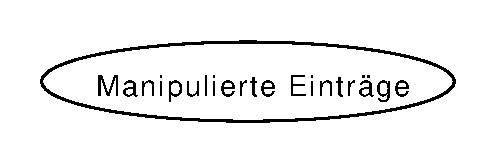
\includegraphics[width=\dimexpr\textwidth-2\tabcolsep-2pt\relax]{../OOA/Use-Case/1-usecase.pdf}

\section{Klassendiagramm}
\subsection{Eintrag}
Das ist unser Datentyp für die Inhalte aus dem Zwischenspeicher. Da wir im
späteren Programmverlauf immer wieder den originalen sowie den modifizierten
brauchen Speichereintrag werden, werden diese Werte in Attributen gespeichert.
Zur Verwaltung ist es zudem immer wieder hilfreich, die Erstellungszeit eines
Objektes zu wissen, um zum Beispiel eine Sortierung zu ermöglichen. Die Klasse
benötigt hierzu keine weiteren Methoden bis auf die Getter und Setter, da sie
nur den Inhalt abbildet.

\subsection{Profil}
Hier werden alle vorgenommen Einstellungen verwaltet. Auch die Parser werden von
dieser Klasse aus verwaltet.  Um verschiedene Einstellungs-Sets parat zu haben
entschieden wir uns mehrere Profile zu ermöglichen. Unterschieden werden diese
über ihren Namen, die der Nutzer festlegt. Ab Werk wird ein „Default“-Profil
angeboten, da ohne ein Profil die Applikation nicht konfiguriert werden kann.
Die Einstellungen die eingeplant sind:
\begin{itemize}
	\item de- / aktivierung eines bestimmten Parsers
	\item de- / aktivierung aller Parser, ohne die einzelnen Parsereinstellungen
zu verändern
\end{itemize}
Ein Profil bietet auch eine Reset-Methode an, um alle Einstellungen zu
verwerfen und mit Defaultwerten zu ersetzen.

\includegraphics[width=\dimexpr\textwidth-2\tabcolsep-2pt\relax]{../OOA/Klassendiagramm/2-klassendiagramm.pdf}

\subsection{Parser}
Das ist das Interface, über das neue Klassen eingebunden werden können. Deren
Zweck ist es Einträge zu modifizieren. Als Beispiel wird eine RegExParser Klasse
erstellt, die ein Such- & Ersetzungsmuster beinhaltet. Optional, sollen diese
Muster auch über eine GUI gesetzt werden können.
Wir haben uns für die Erstellung eines Interfaces entschieden um Plugins zu
ermöglichen, auch wenn der Nutzer nur das bereits kompilierte Programm besitzt.
Da ein Parser später in einer Form dem Nutzer angezeigt werden muss, wird ein
Name und eine Funktionsbeschreibung vorausgesetzt. Da die Grundfunktionalität
die Veränderung von Inhalt ist, ist auch eine Parse-Methode vorgeschrieben.
Optional wird in einem späteren Entwicklungsschritt angepeilt, eine
GUI-Schnittstelle bereitzustellen um dynamischere Manipulationen zuzulassen.

\subsection{Manager}
Der Manager verwaltet die Einträge und die Profile. Hier werden auch die nötigen
Schnittstellen für ein User-Interface bereitgestellt. Außerdem ist der Manager
für die Kommunikation mit dem Betriebssystem zuständig. Dabei wird die
Zwischenablage überprüft, es wird ausgelesen und bei Bedarf verändert.

\section{Aktivitätsdiagramm}
\subsection{Parser bestimmen}
Die Parser sollen dynamisch beim Start des Programms erkannt werden. Ziel ist
es, dem Nutzer zu ermöglichen eigene Parser-Klassen in unserem Paket abzulegen.
Letztendlich können wir nicht alle Einsatzmöglichkeiten voraussehen und halten
das Tool somit flexibel. Bei bedarf kann eine Parser-Suche über ein GUI Element
nochmals gestartet werden, da es sich hierbei um eine Komfortfunktion handelt,
wird diese nur auf Wunsch realisiert.

Zuerst werden alle kompatiblen Parser gesucht, um als kompatibel zu gelten, muss
unser Parser-Interface implementiert sein.

Alle gefundenen Parser werden initialisiert. Danach wird mit dem Profil
abgeglichen ob der Parser derzeit schon aktiv ist.

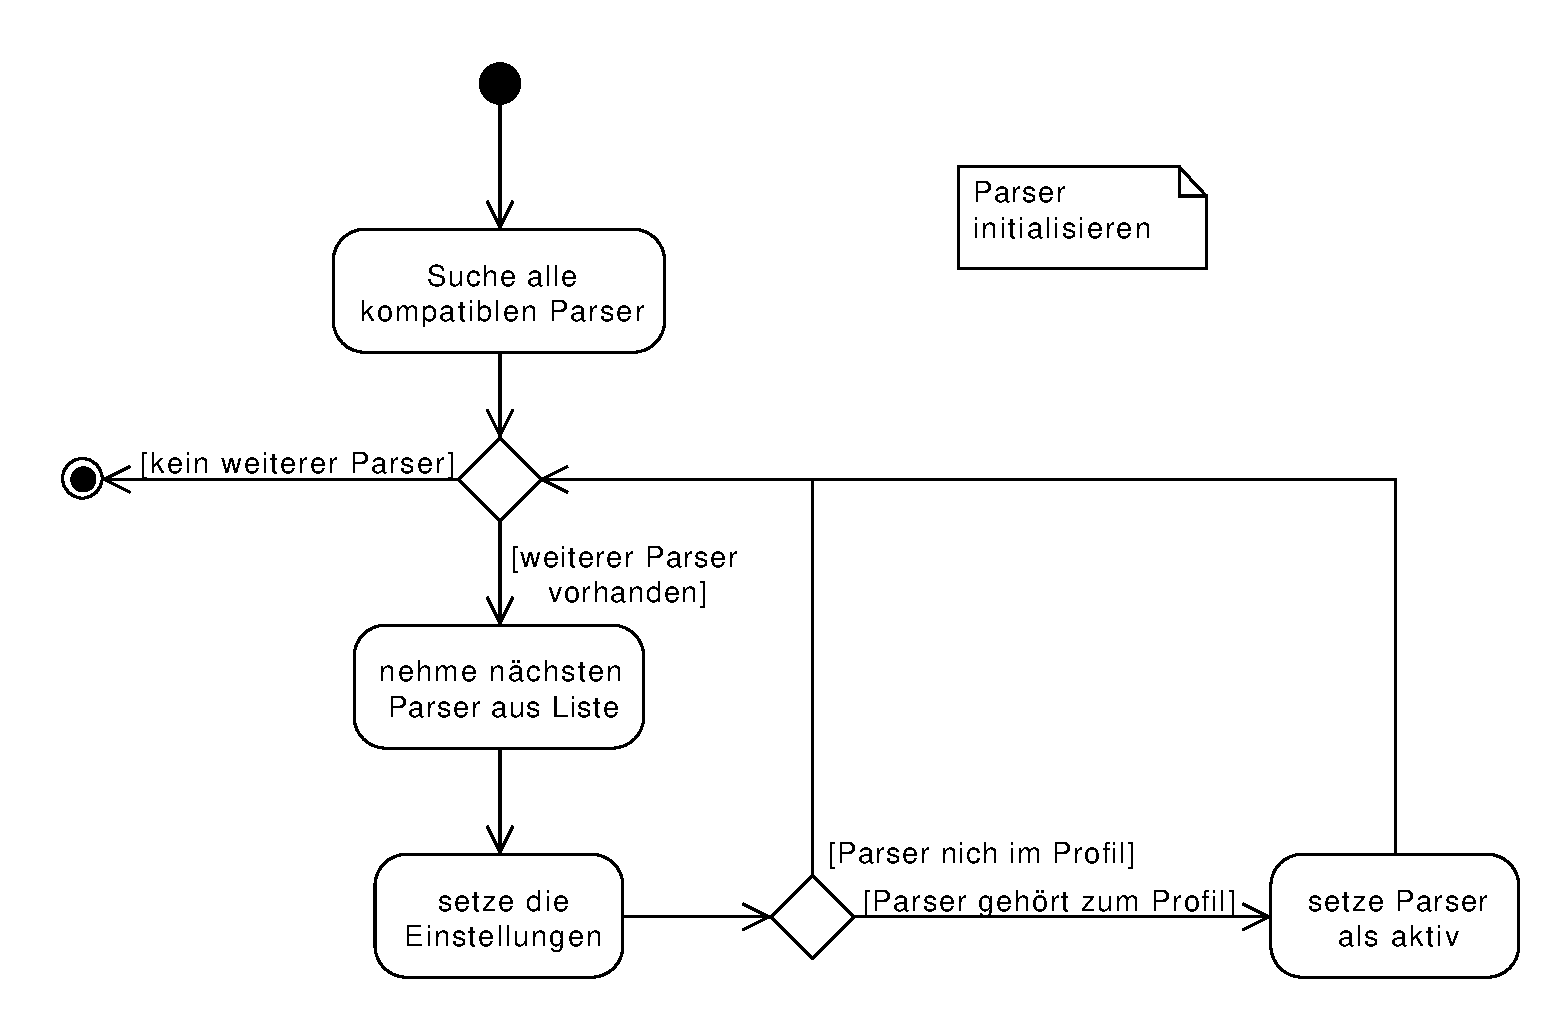
\includegraphics[width=\dimexpr\textwidth-2\tabcolsep-2pt\relax]{../OOA/Aktivitätsdiagramm/1-aktivitydiagramm.pdf}

\subsection{Zwischenablage auslesen}
Die Hauptfunktionalität des Programms, ist es die Zwischenablage zu Verwalten.
Diese wird vom Betriebssystem bereitgestellt und muss über entsprechende
Schnittstellen angesprochen werden. Da dieser Zugriff bereits in Java
implementiert ist, werden wir auf diese Java-Klassen in unserer Darstellung
nicht weiter eingehen. Diesen Vorgang vereinfachen wir auf „Lese Clipboard aus“.

Mit dem Auslesen geht es auch los, der Eintrag wird dem neuesten bekannten
Eintrag verglichen, wenn sie identisch sind, wird der Vorgang beendet. Zur
besseren Veranschaulichung wird in dem Aktivitätsdiagramm die Verbindung zu
„Lese Clipboard aus“ nochmals wiederhergestellt, um die sich immer wiederholende
Aktion darzustellen. Das Programm wartet auf eine Änderung, leider gibt es dafür
keine Ereignisse, also muss die Zwischenablage immer wieder überprüft werden.

Wenn ein neuer Eintrag gefunden wurde, wird dieser in die Liste aufgenommen. 
Wenn der Nutzer allerdings Parser aktiviert hat, wird der Inhalt erst an diese
gereicht. Bei einer Veränderung wird der Inhalt zurück in die Zwischenablage
geschrieben. Die originale Version soll erhalten bleiben.

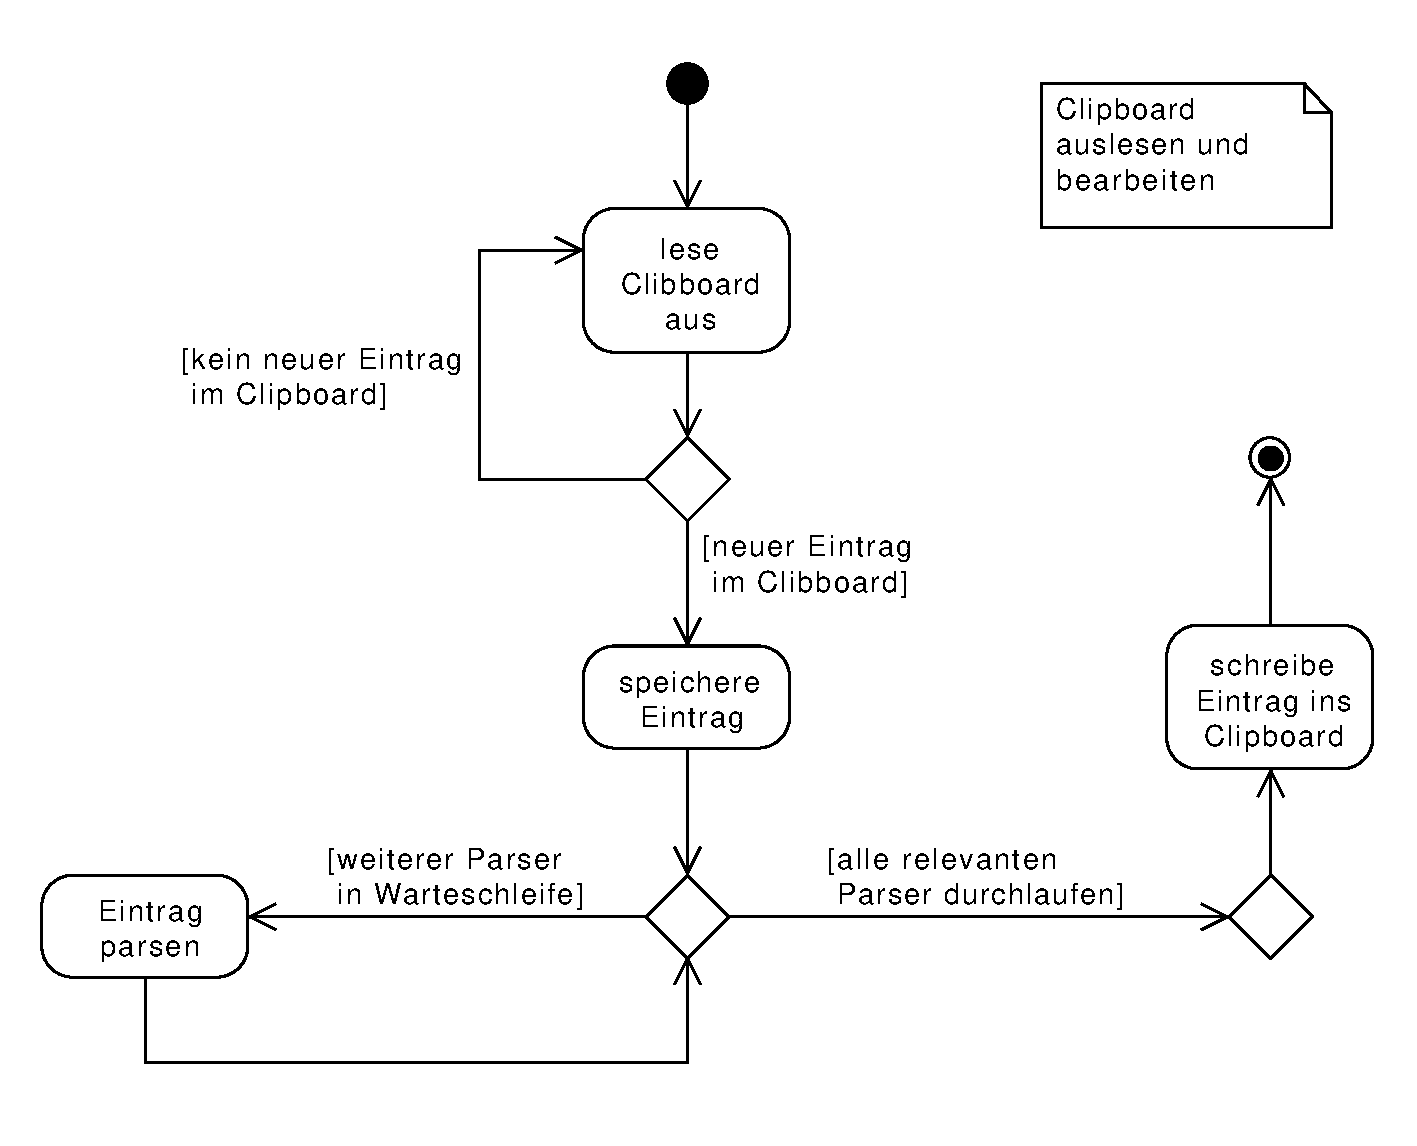
\includegraphics[width=\dimexpr\textwidth-2\tabcolsep-2pt\relax]{../OOA/Aktivitätsdiagramm/2-aktivitydiagramm.pdf}

% Manuelle Layoutänderung, um die Grafiken passend zu den Themen zu plazieren
\newpage

\section{Sequenzdiagramm}
Das Sequenzdiagramm beschreibt das Parsen von neuen Einträgen im Clipboard
während unser Clipboard-Manager ausgeführt wird.

Der Manager überprüft zur Laufzeit in bestimmten Zeitintervallen, ob sich ein
neuer Eintrag im Clipboard befindet. Sobald ein veränderter und/oder neuer
Eintrag registriert wird, erzeugt der Manager ein neues „Eintrag“-Objekt. Danach
holt sich der Manager den Inhalt aus dem Objekt und ruft sein aktuelles Profil
auf. Das aktuelle Profil iteriert über alle für dieses Profil aktiven Parser.
Das bedeutet er parst den Inhalt des neuen Eintrags und schickt ihn an den
Manager zurück. Dieser schreibt die geparsten Daten nun noch in das aktuelle
„Eintrag“-Objekt, damit der neue Inhalt dem User zur Verfügung steht.

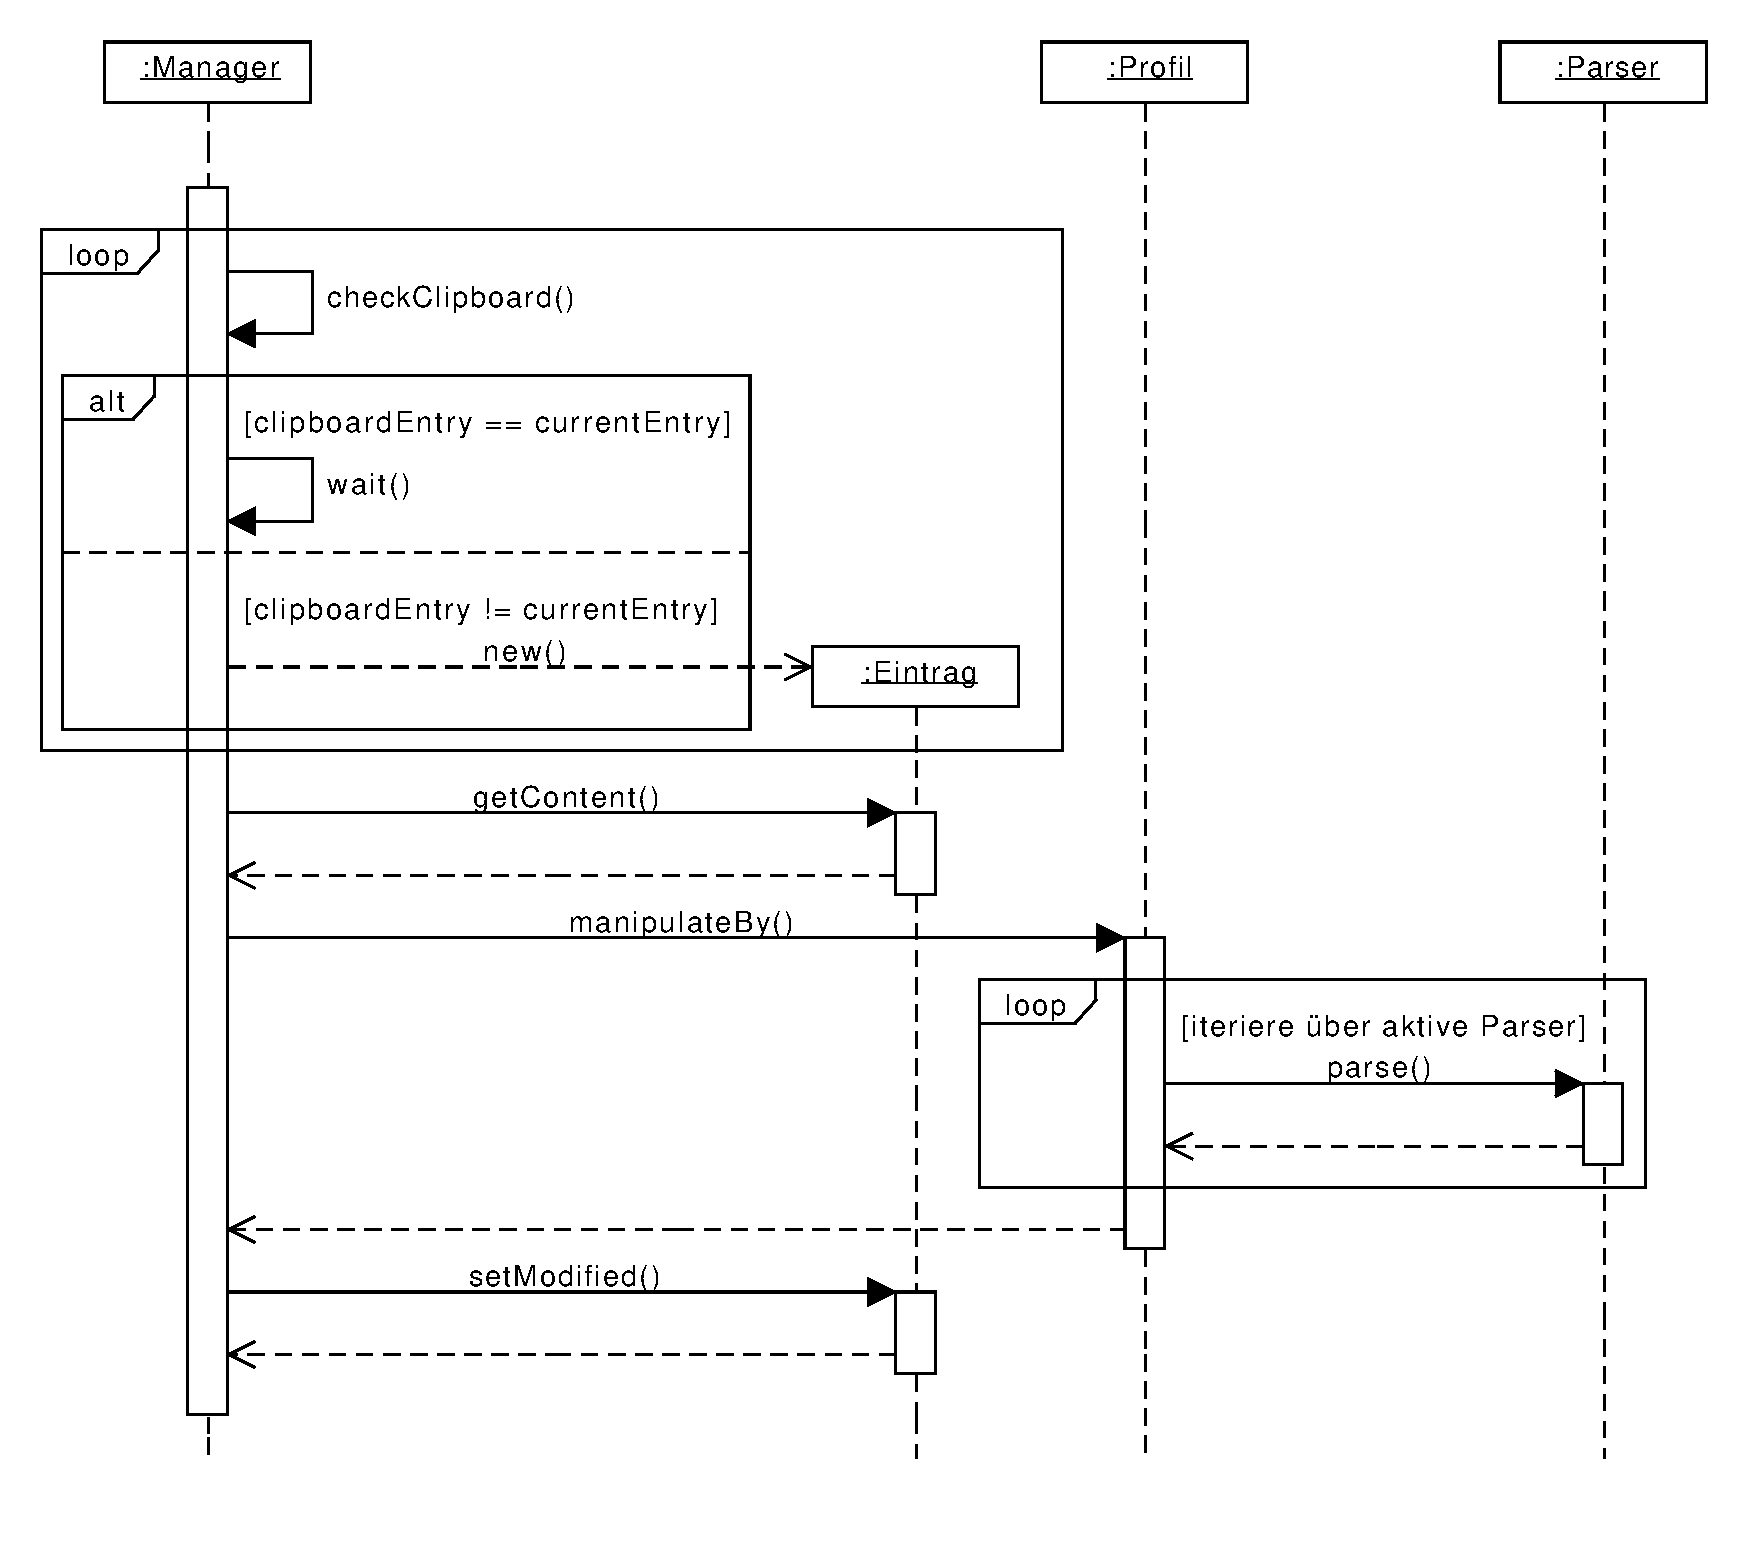
\includegraphics[width=\dimexpr\textwidth-2\tabcolsep-2pt\relax]{../OOA/Sequence/2-sequensdiagramm.pdf}

% Manuelle Layoutänderung, um die Grafiken passend zu den Themen zu plazieren
\newpage

\section{GUI}
\subsection{Standardfenster}
Das Hauptfenster zeigt eine einfache und leichtverständliche Oberfläche, welche
einen Zugang zu allen wichtigen Funktionalitäten bietet, sowie die erfassten
Clipboard-Einträgen auflistet. % so hässlich wie möglich formatiert...
% aber es erfüllt seinen Zweck und stellt die Seite wie gewünscht dar
\\\\
\setlength{\intextsep}{-22pt}
\setlength{\abovecaptionskip}{10pt}
\setlength{\belowcaptionskip}{-10pt}
\begin{wrapfigure}{r}{}
	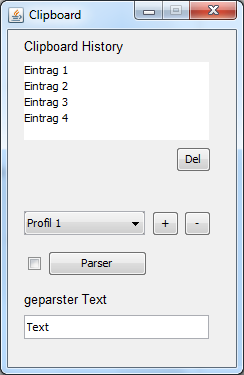
\includegraphics{manager.png}
\end{wrapfigure}
% weiterer Ausrutscher der Formatierungsarbeiten...
\vspace{-45pt}

\begin{enumerate}
	\item In der Clipboard History sieht der Nutzer alle seine Einträge aus
der Zwischenablage. Wenn ein Eintrag ausgewählt wird, wird dieser in die
Zwischenablage geschrieben.
Der Knopf „Del“ löscht den derzeitig ausgewählten Eintrag, dabei wird der
zuletzt aktive Eintrag automatisch ausgewählt, was die selbe Wirkung hat wie die
Auswahl von dem Nutzer.
	\item Im Profilbereich kann ein Profil über ein Dropdown ausgewählt
werden. Dabei werden die gespeicherten Einstellungen geladen.
Der Knopf „+“ bewirkt die Erstellung eines Profils, dabei wird ein
Abfragefenster geöffnet, in dem der Nutzer den Namen des Profils eingeben muss.
„-“ bewirkt im Gegenteil die Löschung des Profils, dies soll auch vom Nutzer
nochmals über eine Abfrage bestätigt werden.

Der Knopf „Parser“ öffnet die Parser Auswahl (siehe unten), die Checkbox stellt die
Manipulation von Einträgen an und aus.
	\item Da der Nutzer auch die Möglichkeit haben soll, seine Parser leicht
einzustellen und zu testen, wird eine Vorschau eingebunden. In dieser wird der
veränderte Eintrag angezeigt.
\end{enumerate}

\begin{wrapfigure}{r}{}
	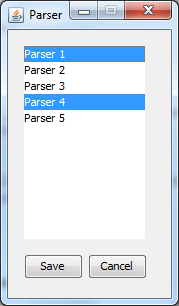
\includegraphics{parser.png}
\end{wrapfigure}

Alle weiteren Funktionaliäten werden in weiteren Dialogen gekapselt und somit
sinnvoll von der Rest des Programms getrennt.

\subsection{Parser Auswahl}
Hier kann der Nutzer über eine Liste die aktiven Parser bestimmen.
In dieser Liste werden alle kompatiblen Parser angezeigt und die aktiven als
Auswahl hervorgehoben.
Beim drücken auf „Save“ werden die Einstellung in das aktive Profil gespeichert.
Bei „Cancel“ wird das Fenster geschlossen (ohne die Einstellungen zu
übernehmen).% Die Zeilenumbrüche gaukeln Latex echte Zeilen am Ende der Seite
%vor, obwohl danach die Seite manuell umgebrochen wird.
\\\\\\\\

\newpage

\section{Ausblick}
Nach der erfolgreichen Objektorientierten Analyse werden wir uns im Weiteren mit
dem genauen Aufbau beschäftigen. Im Zuge dieses Objektorientierten Desings
werden sich gegebenenfalls noch einige Schwächen unseres Entwurfs offenbaren,
aber mit dem bisherigen Prozess ist eine sehr gute Grundlage geschaffen worden
um den Auftrag erfolgreich abzuwickeln. Interessant wird im weiteren Verlauf
außerdem die technische Umsetzung in der Objektorientierten Programmiersprache 
Java.

\end{document}
